\begin{figure}[htp]
   \centering
   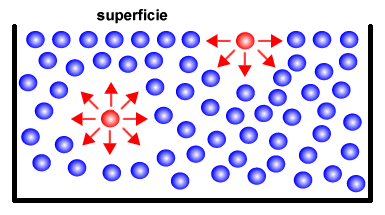
\includegraphics[width=8cm]{immagini/tensione_superficiale.png}
\end{figure}

Consideriamo una generica particella all'interno di un liquido. Essa è sottoposta a varie interazioni in tutte le direzioni, che sono omogenee. 
   
Consideriamo ora una particella che si trova sulla superficie (la superficie in gergo tecnico si chiama \textit{pelo libero del liquido} oppure \textit{interfaccia}). Su di essa si esercitano varie interazioni dovute alle particelle circostanti nella parte interna del liquido, ma altre interazioni mancano, quindi l'entità di interazione su questa particella non sarà la stessa di quella interna.

Se le interazioni che agiscono sulla particella sono attrattive, la particella sulla superficie tenderà ad assumere la forma di una goccia. Dunque, queste interazioni sono responsabili della forma delle superfici dei liquidi.

La tensione superficiale rappresenta il lavoro necessario per aumentare la superficie di un liquido ed è solitamente misurata in $N/m$ oppure in erg per centimetro quadrato $erg/cm^2(=0.001N/m)$. Se usiamo quest'ultima unità di misura, essa rappresenterà il lavoro necessario per aumentare la superficie di un liquido di un centimetro quadrato.

Attenzione! La temperatura ha un ruolo determinante nel modificare l'entità delle interazioni e quindi la tensione superficiale. Pertanto, è importante specificare la temperatura a cui è stata effettuata la misurazione della tensione superficiale.

\hspace{0.5cm}\begin{minipage}{0.395 \textwidth}
   \begin{figure}[H]
       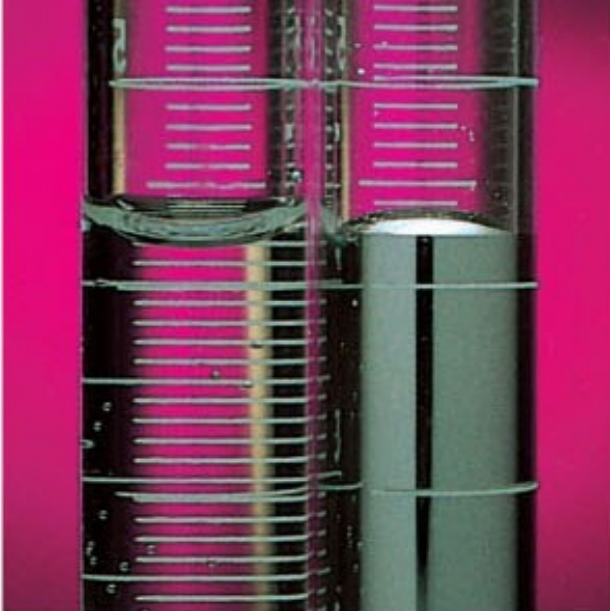
\includegraphics[width=5cm]{immagini/menischi.png}
   \end{figure}
\end{minipage}
\begin{minipage}{0.6 \textwidth}
   \vspace{0.6cm}Abbiamo visto che nei matracci si forma un menisco.
   Questi matracci sono dotati di tacche di 0.1 mL che rappresentano la risoluzione massima. In realtà attraverso le pipette il volume di una tacca può essere diviso in due gocce da 0.05 mL.

   Per determinare il volume di liquido nel matraccio, si legge il valore del menisco inferiore, il quale coincide con la superficie del liquido. È importante leggere il valore della tacca in corrispondenza del centro del menisco, dove la curvatura è meno accentuata.
\end{minipage}

\vspace{0.2cm}La forma del menisco dipende dalla tensione superficiale del liquido e dalla sua adesione alle pareti del recipiente. Nel caso dell'acqua, la sua tensione superficiale è maggiore dell'adesione alle pareti del recipiente, per cui il menisco risulta concavo. Viceversa, nel caso del mercurio, la tensione superficiale è minore dell'adesione alle pareti del recipiente, per cui il menisco risulta convesso.

Quindi la sfericità delle gocce d'acqua dipende dalle interazioni dei legami ad idrogeno.

A questo punto possiamo separare le superfici in due grandi categorie:
\vspace{-0.1cm}
\begin{itemize}
   \item Superfici idrofobiche
   \vspace{-0.1cm}
   \item Superfici idrofile
\end{itemize}

Una superficie idrofobica è una superficie che si bagna poco (respinge l'acqua), perché la sua composizione non interagisce con le molecole dell'acqua. Questo comporta un contatto minimo tra la superficie e l'acqua, che può essere misurato attraverso l'angolo di contatto. In pratica, una goccia d'acqua su una superficie idrofobica mantiene la sua forma sferica.

Al contrario, in una superficie idrofila, l'angolo di contatto è minore di 90 gradi (soltanto qualche grado), il che significa che l'acqua si diffonde sulla superficie.

Le proprietà dell'acqua a contatto con un certo materiale dipendono dalle interazioni tra le molecole del materiale e quelle dell'acqua. 

Inoltre, a causa della tensione superficiale, è possibile che un corpo più denso dell'acqua possa galleggiare sulla sua superficie.